\section{CLS-Pooling}
\begin{figure*}[t]
    \centering
    %\fig[0.45]{method}
    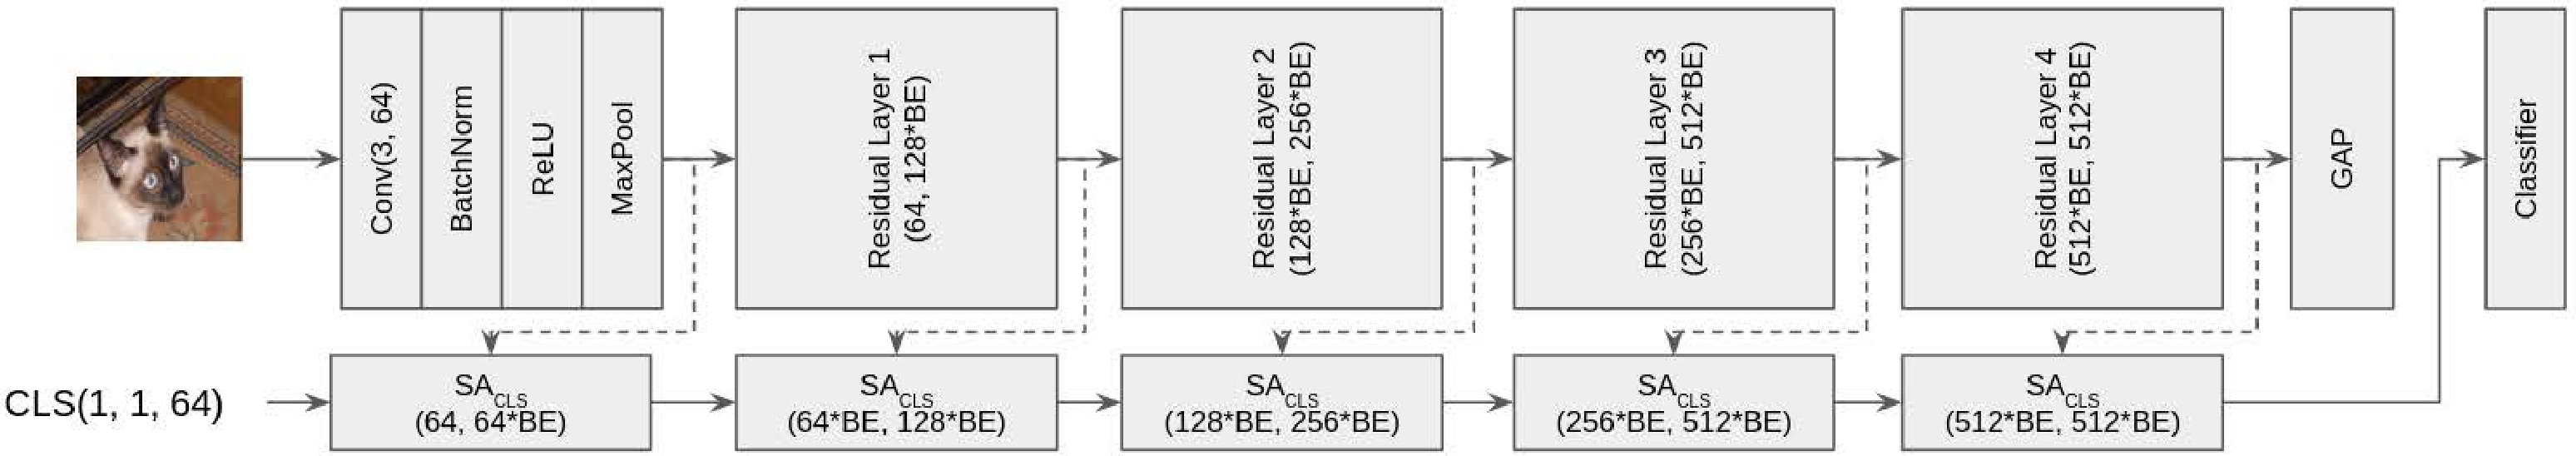
\includegraphics[scale=0.3]{Images/Method/Stream.pdf}
    \caption{Caption}
    \label{fig:fig_method}
\end{figure*}

\subsection{Preliminaries}
\begin{figure}[t]
    \centering
    %\fig[0.45]{method}
    \includegraphics[scale=0.3]{Images/Method/SelfAttention.pdf}
    \caption{Caption}
    \label{fig:fig_crossatt}
\end{figure}
In image classification, our objective is to classify an given image \textit{x}, with the most probable label \textit{y} from the category set $Y=\{y_1, y_2, \dots, y_n\}$. This is done by using an image classification model \textit{f} that can be trained in a supervised or self-supervised way.
\begin{equation}
    y = f(x)
\end{equation}
Assuming this model \textit{f} is made up from a sequence of operations (or layers), it is possible to dissect it at different depths \textit{k} and observe the representation $F_k$ of this given image in this space.
\begin{equation}
    F_k = f_k(F_{k-1})
\end{equation}
On another hand, it is feasible to make use of a classification token ({[class]}) \cite{DBLP:journals/corr/abs-1810-04805,DBLP:journals/corr/abs-2010-11929} that is used as an image representation to be used towards this task. In prior approaches, this token is prepended to the patch embedding of \textit{x}; whereas  in this approach, we aim at learning this representation by leveraging the interactions with feature maps at given points of a network. %Therefore, this token $Q$ is updated alongside \textit{F} at different depths of the network.

\subsection{Cross-Attention module}
Taking inspiration from \cite{DBLP:journals/corr/ChengDL16}; we devise a cross attention module (CA) that is built upon the sequential property of CNNs, to update a global image representation $Q$. To do so, in comparison to self attention; we compute the similarity between this representation and the feature maps for a given point. We preserve the scaling factor proposed in \cite{NIPS2017_3f5ee243} as the dimension of feature maps increases alongside depth; therefore the dimension of this representation is increased as well.
\begin{equation}
    \mbox{CA}_k(Q_{k}, F_{k+1}) = \mbox{softmax}(\frac{Q_{k}F^T_{k+1}}{\sqrt{dim_k}})F_{k+1}
\end{equation}
This class token is initialized with a normal distribution \ref{eq:qinit}, and is updated across given points in the network with the features found in the following stage. Conversely, as the feature maps width is increased alongside the depth of the network, we make use of a linear projection \textit{W} to allow our representation to interact with said features at different depths of \textit{f} \ref{eq:qklayer}.
% the width of our representation is increased via linear projection \textit{W} on top of the attention mechanism. %Our cross attention module is presented in figure \ref{fig:fig_crossatt}\\
\begin{equation}
    Q_0 \sim \mathcal{N}(1, 1) 
    \label{eq:qinit}
\end{equation}
\begin{equation}    
    Q_{k+1} = W_k(\mbox{CA}_{k}(Q_{k}, F_{k}))
    \label{eq:qklayer}
\end{equation}
Our Cross Attention model is summarized on figure \ref{fig:fig_crossatt}


\subsection{Cross-Attention Stream}
Taking into consideration this proposed attention module, we observe that it can be applied at different stages of \textit{f}. In particular, we focus on depths where changes in the area of feature maps gets reduced by pooling operations. Conversely, ever since its proposal GAP\cite{lin2013network} has been used to rely information from feature maps into the classifier stages for CNNs; however since this pooling approach is uniform, the representation observed by these operations does not completely convey the real contribution of certain image patches towards our classification task. To alleviate this, we utilize our {[class]} token to update the representation examined at earlier points in the model, while also pooling the features found in the latest convolutional block of \textit{f}. An example of this stream can be observed in figure \ref{fig:fig_method} where it is applied to a ResNet based architecture. 

